\documentclass[11pt,openany]{book}
\usepackage[]{graphicx}\usepackage[]{color}
%% maxwidth is the original width if it is less than linewidth
%% otherwise use linewidth (to make sure the graphics do not exceed the margin)
\makeatletter
\def\maxwidth{ %
  \ifdim\Gin@nat@width>\linewidth
    \linewidth
  \else
    \Gin@nat@width
  \fi
}
\makeatother

\definecolor{fgcolor}{rgb}{0.345, 0.345, 0.345}
\newcommand{\hlnum}[1]{\textcolor[rgb]{0.686,0.059,0.569}{#1}}%
\newcommand{\hlstr}[1]{\textcolor[rgb]{0.192,0.494,0.8}{#1}}%
\newcommand{\hlcom}[1]{\textcolor[rgb]{0.678,0.584,0.686}{\textit{#1}}}%
\newcommand{\hlopt}[1]{\textcolor[rgb]{0,0,0}{#1}}%
\newcommand{\hlstd}[1]{\textcolor[rgb]{0.345,0.345,0.345}{#1}}%
\newcommand{\hlkwa}[1]{\textcolor[rgb]{0.161,0.373,0.58}{\textbf{#1}}}%
\newcommand{\hlkwb}[1]{\textcolor[rgb]{0.69,0.353,0.396}{#1}}%
\newcommand{\hlkwc}[1]{\textcolor[rgb]{0.333,0.667,0.333}{#1}}%
\newcommand{\hlkwd}[1]{\textcolor[rgb]{0.737,0.353,0.396}{\textbf{#1}}}%
\let\hlipl\hlkwb

\usepackage{framed}
\makeatletter
\newenvironment{kframe}{%
 \def\at@end@of@kframe{}%
 \ifinner\ifhmode%
  \def\at@end@of@kframe{\end{minipage}}%
  \begin{minipage}{\columnwidth}%
 \fi\fi%
 \def\FrameCommand##1{\hskip\@totalleftmargin \hskip-\fboxsep
 \colorbox{shadecolor}{##1}\hskip-\fboxsep
     % There is no \\@totalrightmargin, so:
     \hskip-\linewidth \hskip-\@totalleftmargin \hskip\columnwidth}%
 \MakeFramed {\advance\hsize-\width
   \@totalleftmargin\z@ \linewidth\hsize
   \@setminipage}}%
 {\par\unskip\endMakeFramed%
 \at@end@of@kframe}
\makeatother

\definecolor{shadecolor}{rgb}{.97, .97, .97}
\definecolor{messagecolor}{rgb}{0, 0, 0}
\definecolor{warningcolor}{rgb}{1, 0, 1}
\definecolor{errorcolor}{rgb}{1, 0, 0}
\newenvironment{knitrout}{}{} % an empty environment to be redefined in TeX

\usepackage{alltt}
\newcommand{\SweaveOpts}[1]{}  % do not interfere with LaTeX
\newcommand{\SweaveInput}[1]{} % because they are not real TeX commands
\newcommand{\Sexpr}[1]{}       % will only be parsed by R


\usepackage[utf8]{inputenc} 
\usepackage{amssymb, amsmath, amsthm}
\usepackage{fullpage}
\usepackage{setspace}
\usepackage{graphicx}
\usepackage{natbib}
\usepackage{rotating}
\usepackage{caption}
\usepackage{subcaption}
\usepackage{multirow}
\usepackage{booktabs}
\usepackage{dcolumn}
\usepackage[grey]{quotchap}
\usepackage{xcolor}
\usepackage[left=1in, top=1in, right=1.5in, bottom=1in, headsep=.5in]
{geometry}
\usepackage{fancyhdr, blindtext}
\usepackage{diagbox}
\usepackage{hyperref} 
\usepackage{placeins}
\renewenvironment{knitrout}{\begin{singlespace}}{\end{singlespace}}
\newcommand*{\mybox}[2]{\colorbox{#1!30}{\parbox{.98\linewidth}{#2}}}
\newcommand*{\befehl}[1]{\texttt{\textbackslash #1}} % Added by 


\fancyhf{}
\fancyhead[LE]{\slshape \rightmark} 
\fancyhead[RE]{\thepage}
\fancyhead[RO]{\slshape \leftmark} 
\fancyhead[LO]{\thepage}
\renewcommand{\headrulewidth}{0.4pt}
\pagestyle{fancy}
%% new command for greybox
\long\def\greybox#1{%
    \newbox\contentbox%
    \newbox\bkgdbox%
    \setbox\contentbox\hbox to \hsize{%
        \vtop{
            \kern\columnsep
            \hbox to \hsize{%
                \kern\columnsep%
                \advance\hsize by -2\columnsep%
                \setlength{\textwidth}{\hsize}%
                \vbox{
                    \parskip=\baselineskip
                    \parindent=0bp
                    #1
                }%
                \kern\columnsep%
            }%
            \kern\columnsep%
        }%
    }%
    \setbox\bkgdbox\vbox{
        \pdfliteral{0.85 0.85 0.85 rg}
        \hrule width  \wd\contentbox %
               height \ht\contentbox %
               depth  \dp\contentbox
        \pdfliteral{0 0 0 rg}
    }%
    \wd\bkgdbox=0bp%
    \vbox{\hbox to \hsize{\box\bkgdbox\box\contentbox}}%
    \vskip\baselineskip%
}
%% make greybox (grbox) a float
\usepackage{float}
\newfloat{grbox}{thp}{lop}[section]
\floatname{grbox}{Grey Box}



\begin{document}




\chapter{Bi-Variate Hypothesis Testing and Model Fit}

The previous chapters discussed the logic of OLS regression and how to derive OLS estimators. Now that simple regression is no longer a mystery, we will shift the focus to bi-variate hypothesis testing and model fit. Note that the examples in this chapter use the \texttt{tbur} data set.  We recommend that you try the analyses in the chapter as you read.

\section{Hypothesis Tests for Regression Coefficients}

Hypothesis testing is the key to theory building. This chapter is focused on empirical hypothesis testing using OLS regression, using examples drawn from the accompanying dataset (tbur.data). Here we will use the responses to the political ideology question  (ranging from 1=strong liberal, to 7=strong conservative), as well as responses to a question concerning the survey respondents' level of risk that global warming poses for people and the environment.\footnote{The question wording was as follows: ``On a scale from zero to ten, where zero
means no risk and ten means extreme risk, how much
risk do you think global warming poses for people
and the environment?"}

Using the data from these questions, we posit the following hypothesis:
\begin{quote}
$H_{1}$: On average, as respondents, become more politically conservative, they will be less likely to express increased risk associated with global warming.
\end{quote}

The null hypothesis, $H_{0}$, is $\beta = 0$, positing that a respondents ideology has no relationship with their views about the risks of global warming for people and the environment. Our working hypothesis, $H_{1}$, is $\beta < 0$. We expect $\beta$ to be less than zero because we expect a \textit{negative} slope between our measures of ideology and levels of risk associated with global warming, given that a larger numeric value for ideology indicates a more conservative respondent. Note that this is a \textit{directional} hypothesis since we are positing a negative relationship. Typically, a directional hypothesis implies a one-tailed test where the critical value is 0.05 on one side of the distribution. A \textit{non-directional} hypothesis, $\beta \neq 0$ does not imply a particular direction, it only implies that there is a relationship. This requires a two-tailed test where the critical value is 0.025 on both sides of the distribution.  

To test this hypothesis, we run the following code in \texttt{R}. 

Before we begin, for this chapter, we need to make a special data set that just contains the variables \texttt{glbccrisk} and \texttt{ideol} with missing values removed.

\begin{knitrout}
\definecolor{shadecolor}{rgb}{0.969, 0.969, 0.969}\color{fgcolor}\begin{kframe}
\begin{alltt}
\hlcom{#Filtering a data set with only variables glbcc_risk and ideol}
\hlstd{ds.omit} \hlkwb{<-} \hlkwd{filter}\hlstd{(ds)} \hlopt
  \hlkwd{select}\hlstd{(glbcc_risk,ideol)} \hlopt
  \hlkwd{na.omit}\hlstd{()}
\hlcom{#Run the na.omit function to removed the value}
\end{alltt}
\end{kframe}
\end{knitrout}


\begin{knitrout}
\definecolor{shadecolor}{rgb}{0.969, 0.969, 0.969}\color{fgcolor}\begin{kframe}
\begin{alltt}
\hlstd{ols1} \hlkwb{<-} \hlkwd{lm}\hlstd{(glbcc_risk} \hlopt{~} \hlstd{ideol,} \hlkwc{data} \hlstd{= ds.omit)}
\hlkwd{summary}\hlstd{(ols1)}
\end{alltt}
\begin{verbatim}
## 
## Call:
## lm(formula = glbcc_risk ~ ideol, data = ds.omit)
## 
## Residuals:
##    Min     1Q Median     3Q    Max 
## -8.726 -1.633  0.274  1.459  6.506 
## 
## Coefficients:
##             Estimate Std. Error t value Pr(>|t|)    
## (Intercept) 10.81866    0.14189   76.25   <2e-16 ***
## ideol       -1.04635    0.02856  -36.63   <2e-16 ***
## ---
## Signif. codes:  0 '***' 0.001 '**' 0.01 '*' 0.05 '.' 0.1 ' ' 1
## 
## Residual standard error: 2.479 on 2511 degrees of freedom
## Multiple R-squared:  0.3483,	Adjusted R-squared:  0.348 
## F-statistic:  1342 on 1 and 2511 DF,  p-value: < 2.2e-16
\end{verbatim}
\end{kframe}
\end{knitrout}

To know whether to accept of reject the null hypothesis, we need to first understand the standard error associated with the model and our coefficients. We start, therefore, with  consideration of the residual standard error of the regression model. 

\subsection{Residual Standard Error} 

The residual standard error (or standard error of the regression),  measures spread of our observations around the regression line. As will be discussed below, the residual standard error is used to calculate the standard errors of the regression coefficients, $A$ and $B$. 

The formula for the residual standard error is as follows:
\begin{equation}
S_{E}=\sqrt{\frac{\Sigma E^{2}_{i}}{n-2}}
\end{equation}

To calculate this in \texttt{R}, based on the model we just ran,  we create an object called \texttt{Se} and use the \texttt{sqrt} and \texttt{sum} commands. 
\begin{knitrout}
\definecolor{shadecolor}{rgb}{0.969, 0.969, 0.969}\color{fgcolor}\begin{kframe}
\begin{alltt}
\hlstd{Se} \hlkwb{<-} \hlkwd{sqrt}\hlstd{(}\hlkwd{sum}\hlstd{(ols1}\hlopt{$}\hlstd{residuals}\hlopt{^}\hlnum{2}\hlstd{)}\hlopt{/}\hlstd{(}\hlkwd{length}\hlstd{(ds.omit}\hlopt{$}\hlstd{glbcc_risk)}\hlopt{-}\hlnum{2}\hlstd{))}
\hlstd{Se}
\end{alltt}
\begin{verbatim}
## [1] 2.479022
\end{verbatim}
\end{kframe}
\end{knitrout}
\noindent Note that this result matches the result provided by the \texttt{summary} function in \texttt{R}, as shown above.  

For our model, the results indicate that: $Y_{i} =$ 10.8186624 -1.0463463$X_{i} + E_{i}$.  Another sample of 2513 observations would almost certainly lead to different estimates for $A$ and $B$.  If we drew many such samples, we’d get the sample distribution of the estimates. Because we typically cannot draw many samples, we need to estimate the sample distribution, based on our sample size and variance.  To do that, we calculate the standard error of the slope and intercept coefficients, $SE(B)$ and $SE(A)$. These standard errors are our estimates of how much variation we would expect in the estimates of $B$ and $A$ across different samples. We use them to evaluate whether $B$ and $A$ are larger that would be expected to occur by chance, if the real values of $B$ and/or $A$ are zero (the null hypotheses).

The standard error for $B$, $SE(B)$ is:
\begin{equation}
SE(B)=\frac{S_{E}}{\sqrt{TSS_{X}}}
\end{equation}
\noindent where $S_E$ is the residual standard error of the regression, (as whown earlier in equation 9.1). $TSS_X$ is the total sum of squares for $X$, that is the total sum of the squared deviations (residuals) of $X$ from its mean $\bar{X}$; $\sum (X_i-\bar{X})^{2}$. Note that the greater the deviation of $X$ around its mean as a proportion of the standard error of the model, the smaller the $SE(B)$. The smaller $SE(B)$ is, the less variation we would expect in repeated estimates of $B$ across multiple samples.

The standard error for $A$, $SE(A)$, is defined as:
\begin{equation}
SE(A)=S_{E}*\sqrt{\frac{1}{n}+\frac{\bar X^{2}}{TSS_{X}}}
\end{equation}

Again, the $SE$ is the residual standard error, as shown in equation 9.1.

\noindent For $A$, the larger the data set, and the larger the deviation of $X$ around its mean, the more precise our estimate of $A$ (i.e., the smaller $SE(A)$ will be).  

We can calculate the $SE$ of $A$ and $B$ in \texttt{R} in a few steps. First, we create an object \texttt{TSSx} that is the total sum of squares for the $X$ variable. 

\begin{knitrout}
\definecolor{shadecolor}{rgb}{0.969, 0.969, 0.969}\color{fgcolor}\begin{kframe}
\begin{alltt}
\hlstd{TSSx} \hlkwb{<-} \hlkwd{sum}\hlstd{((ds.omit}\hlopt{$}\hlstd{ideol}\hlopt{-}\hlkwd{mean}\hlstd{(ds.omit}\hlopt{$}\hlstd{ideol,} \hlkwc{na.rm} \hlstd{=} \hlnum{TRUE}\hlstd{))}\hlopt{^}\hlnum{2}\hlstd{)}
\hlstd{TSSx}
\end{alltt}
\begin{verbatim}
## [1] 7532.946
\end{verbatim}
\end{kframe}
\end{knitrout}

\noindent Then, we create an object called \texttt{SEa}.
\begin{knitrout}
\definecolor{shadecolor}{rgb}{0.969, 0.969, 0.969}\color{fgcolor}\begin{kframe}
\begin{alltt}
\hlstd{SEa} \hlkwb{<-} \hlstd{Se}\hlopt{*}\hlkwd{sqrt}\hlstd{((}\hlnum{1}\hlopt{/}\hlkwd{length}\hlstd{(ds.omit}\hlopt{$}\hlstd{glbcc_risk))}\hlopt{+}\hlstd{(}\hlkwd{mean}\hlstd{(ds.omit}\hlopt{$}\hlstd{ideol,}\hlkwc{na.rm}\hlstd{=T)}\hlopt{^}\hlnum{2}\hlopt{/}\hlstd{TSSx))}
\hlstd{SEa}
\end{alltt}
\begin{verbatim}
## [1] 0.1418895
\end{verbatim}
\end{kframe}
\end{knitrout}

\noindent Finally, we create  \texttt{SEb}.
\begin{knitrout}
\definecolor{shadecolor}{rgb}{0.969, 0.969, 0.969}\color{fgcolor}\begin{kframe}
\begin{alltt}
\hlstd{SEb} \hlkwb{<-} \hlstd{Se}\hlopt{/}\hlstd{(}\hlkwd{sqrt}\hlstd{(TSSx))}
\hlstd{SEb}
\end{alltt}
\begin{verbatim}
## [1] 0.02856262
\end{verbatim}
\end{kframe}
\end{knitrout}

Using the standard errors, we can determine how likely it is that our estimate of $\beta$ differs from $0$; that is how many standard errors our estimate is away from $0$. To determine this we use the $t$ value. The $t$ score is derived by dividing the regression coefficient by its standard error. For our model, the $t$ value for $\beta$ is as follows: 
\begin{knitrout}
\definecolor{shadecolor}{rgb}{0.969, 0.969, 0.969}\color{fgcolor}\begin{kframe}
\begin{alltt}
\hlstd{t} \hlkwb{<-} \hlstd{ols1}\hlopt{$}\hlstd{coef[}\hlnum{2}\hlstd{]}\hlopt{/}\hlstd{SEb}
\hlstd{t}
\end{alltt}
\begin{verbatim}
##     ideol 
## -36.63342
\end{verbatim}
\end{kframe}
\end{knitrout}

The $t$ value for our $B$ is -36.6334214, meaning that $B$ is -36.6334214 standard errors away from zero. We can then ask: What is the probability, $p$ \textit{value}, of obtaining this result if $\beta=0$? According to the results shown earlier, $p=2e-16$. That is remarkably close to zero. This result indicates that we can reject the null hypothesis
that $\beta=0$. 

In addition, we can calculate the confidence interval (CI) for our estimate of $B$.  This means that in 95 out of 100 repeated applications, the confidence interval will contain $\beta$. 

In the following example, we calculate a $95\%$ CI. The CI is calculated as follows: 
\begin{equation}
  \label{eq:ci}
  B \pm 1.96(SE(B))
\end{equation}

We can easily calculate this in \texttt{R}. First, we calculate the upper limit then the lower limit and then we use the \texttt{confint} function to check.   
\begin{knitrout}
\definecolor{shadecolor}{rgb}{0.969, 0.969, 0.969}\color{fgcolor}\begin{kframe}
\begin{alltt}
\hlstd{Bhi} \hlkwb{<-} \hlstd{ols1}\hlopt{$}\hlstd{coef[}\hlnum{2}\hlstd{]}\hlopt{-}\hlnum{1.96}\hlopt{*}\hlstd{SEb}
\hlstd{Bhi}
\end{alltt}
\begin{verbatim}
##     ideol 
## -1.102329
\end{verbatim}
\begin{alltt}
\hlstd{Blow} \hlkwb{<-} \hlstd{ols1}\hlopt{$}\hlstd{coef[}\hlnum{2}\hlstd{]}\hlopt{+}\hlnum{1.96}\hlopt{*}\hlstd{SEb}
\hlstd{Blow}
\end{alltt}
\begin{verbatim}
##      ideol 
## -0.9903636
\end{verbatim}
\begin{alltt}
\hlkwd{confint}\hlstd{(ols1)}
\end{alltt}
\begin{verbatim}
##                 2.5 %     97.5 %
## (Intercept) 10.540430 11.0968947
## ideol       -1.102355 -0.9903377
\end{verbatim}
\end{kframe}
\end{knitrout}

As shown, the upper limit of our estimated $B$ is -0.9903636, which is far below $0$, providing further support for rejecting $H_0$. 

So, using our example data, we tested the working hypothesis that political ideology is negatively related to expressed risk of global warming to people and the environment. Using simple OLS regression, we find support for that working hypothesis, and can reject the null.

\section{Measuring Goodness of Fit}

Once we have constructed a regression model, it is natural to ask: how \texttt{good} is the model at explaining variation in our dependent variable? We answer this question with a number of statistics that indicate ``model fit". Basically, these statistics provide measures of the degree to which the estimated relationships account for the variance in the dependent variable, $Y$.

There are several ways to examine how well the model ``explains" the variance in $Y$. First, we can examine the covariance of $X$ and $Y$, which is a general measure of the sample variance for $X$ and $Y$. Then we can use a measure of sample \texttt{correlation}, which is the standardized measure of covariation. Both of these measures provide indicators of the degree to which variation in $X$ can account for variation in $Y$. Finally, we can examine $R^{2}$, also know as the coefficient of determination, which is the standard measure of the goodness of fit for OLS models. 

\subsection{Sample Covariance and Correlations}
 
The sample covariance for a simple regression model is defined as:
\begin{equation}
S_{XY} = \frac {\Sigma(X_{i}-\bar X)(Y_{i}-\bar Y)}{n-1}
\end{equation}
Intuitively, this measure tells you, on average, whether a higher value of $X$ (relative to its mean) is associated with a higher or lower value of $Y$. Is the association negative or positive? Covariance can be obtained quite simply in \texttt{R} by using the the \texttt{cov} function.
\begin{knitrout}
\definecolor{shadecolor}{rgb}{0.969, 0.969, 0.969}\color{fgcolor}\begin{kframe}
\begin{alltt}
\hlstd{Sxy} \hlkwb{<-} \hlkwd{cov}\hlstd{(ds.omit}\hlopt{$}\hlstd{ideol, ds.omit}\hlopt{$}\hlstd{glbcc_risk)}
\hlstd{Sxy}
\end{alltt}
\begin{verbatim}
## [1] -3.137767
\end{verbatim}
\end{kframe}
\end{knitrout}

The problem with covariance is that its magnitude will be entirely dependent on the scales used to measure $X$ and $Y$. That is, it is non-standard, and its meaning will vary depending on what it is that is being measured. In order to compare sample covariation across different samples and different measures, we use the sample \texttt{correlation}.

The sample correlation, $r$, is found by dividing $S_{XY}$ by the product of the standard deviations of $X$, $S_{X}$, and $Y$, $S_{Y}$. 

\begin{equation}
r=\frac{S_{XY}}{S_{X}S_{Y}}=\frac{\Sigma(X_{i}-\bar{X})(Y_{i}-\bar
  Y)}{\sqrt{\Sigma(X_{i}-\bar X)^{2} \Sigma(Y_{i}-\bar Y)^{2}}} 
\end{equation}

To calculate this in \texttt{R}, we first make an object for $S_{X}$ and $S_{Y}$ using the \texttt{sd} function. 
\begin{knitrout}
\definecolor{shadecolor}{rgb}{0.969, 0.969, 0.969}\color{fgcolor}\begin{kframe}
\begin{alltt}
\hlstd{Sx} \hlkwb{<-} \hlkwd{sd}\hlstd{(ds.omit}\hlopt{$}\hlstd{ideol)}
\hlstd{Sx}
\end{alltt}
\begin{verbatim}
## [1] 1.7317
\end{verbatim}
\begin{alltt}
\hlstd{Sy} \hlkwb{<-} \hlkwd{sd}\hlstd{(ds.omit}\hlopt{$}\hlstd{glbcc_risk)}
\hlstd{Sy}
\end{alltt}
\begin{verbatim}
## [1] 3.070227
\end{verbatim}
\end{kframe}
\end{knitrout}
\noindent Then to find $r$:
\begin{knitrout}
\definecolor{shadecolor}{rgb}{0.969, 0.969, 0.969}\color{fgcolor}\begin{kframe}
\begin{alltt}
\hlstd{r} \hlkwb{<-} \hlstd{Sxy}\hlopt{/}\hlstd{(Sx}\hlopt{*}\hlstd{Sy)}
\hlstd{r}
\end{alltt}
\begin{verbatim}
## [1] -0.5901706
\end{verbatim}
\end{kframe}
\end{knitrout}
\noindent To check this we can use the \texttt{cor} function in \texttt{R}. 
\begin{knitrout}
\definecolor{shadecolor}{rgb}{0.969, 0.969, 0.969}\color{fgcolor}\begin{kframe}
\begin{alltt}
\hlstd{rbyR} \hlkwb{<-} \hlkwd{cor}\hlstd{(ds.omit}\hlopt{$}\hlstd{ideol, ds.omit}\hlopt{$}\hlstd{glbcc_risk)}
\hlstd{rbyR}
\end{alltt}
\begin{verbatim}
## [1] -0.5901706
\end{verbatim}
\end{kframe}
\end{knitrout}

So what does the correlation coefficient mean? The values range from +1 to -1, and a value of +1 means  there is a perfect positive relationship between $X$ and $Y$. Each increment of increase in $X$ is matched by a constant increase in $Y$ -- with all observations lining up neatly on a positive slope. A correlation  coefficient of -1, a perfect negative relationship, would indicate that each increment of increase in $X$ corresponds to a constant decrease in $Y$ -- or a negatively sloped line. A correlation coefficient of zero would describe \texttt{no relationship} between $X$ and $Y$.

\subsection{Coefficient of Determination: $R^{2}$} 

The most often used measure of goodness of fit for OLS models is $R^{2}$.  $R^{2}$ is derived from three components; the total sum of squares, the explained sum of squares, and the residual sum of squares. $R^{2}$ is the ratio of \textbf{ESS} (explained sum of squares) to \textbf{TSS} (total sum of squares).
 
\begin{grbox}
\greybox{\textbf{Components of $R^{2}$}
\begin{itemize}  
\item \textit{Total sum of squares (TSS)}: The
sum of the squared variance of $Y$ 
\begin{center}
  $\sum E'^{2}_{i} = \sum (Y-\bar{Y})^{2}$
\end{center}
\item \textit{Residual sum of squares(RSS)}: The variance of $Y$ not
  accounted for by the model  
  \begin{center}
  $\sum E^{2}_{i} = \sum (Y-\hat{Y})^{2} = \sum (Y_{i}-A-BX_{i})^{2}$    
  \end{center}
\item \textit{Explained sum of squares (ESS)}: The variance of $Y$
  accounted for in the model
  
\noindent It is the difference between the TSS and the RSS.
  
  \begin{center}
  $ESS = TSS-RSS$  
  \end{center}
\item \textit{$R^{2}$}: The proportion of the total
  variance of $Y$ explained by the model
  %it is the ratio of $ESS$ to
  %$TSS$ 
  \begin{align*}
  R^{2} &= \frac{ESS}{TSS} \\
  \\
  &= \frac{TSS-RSS}{TSS} \\
  \\
  &= 1-\frac{RSS}{TSS}
  \end{align*}   
\end{itemize}}
\end{grbox} 
% insert figure from slides 

The components of $R^{2}$ are illustrated in Figure \ref{fig:rsquared}. As shown, for each observation $Y_{i}$, variation around the mean can be decomposed into that which is ``explained" by the regression and that which is not. In Figure \ref{fig:rsquared}, the deviation between the mean of $Y$ and the predicted value of $Y$, $\hat{Y}$, is the proportion of the variation of  $Y_{i}$ that can be explained (or predicted) by the regression. That is shown as a blue line. The deviation of the observed value of $Y_{i}$ from the predicted value $\hat{Y}$ (aka the residual, as discussed in the previous chapter) is the unexplained deviation, shown in red. Together, the explained and unexplained variation make up the total variation of  $Y_{i}$ around the mean $\hat{Y}$.

\begin{figure}
  \centering
  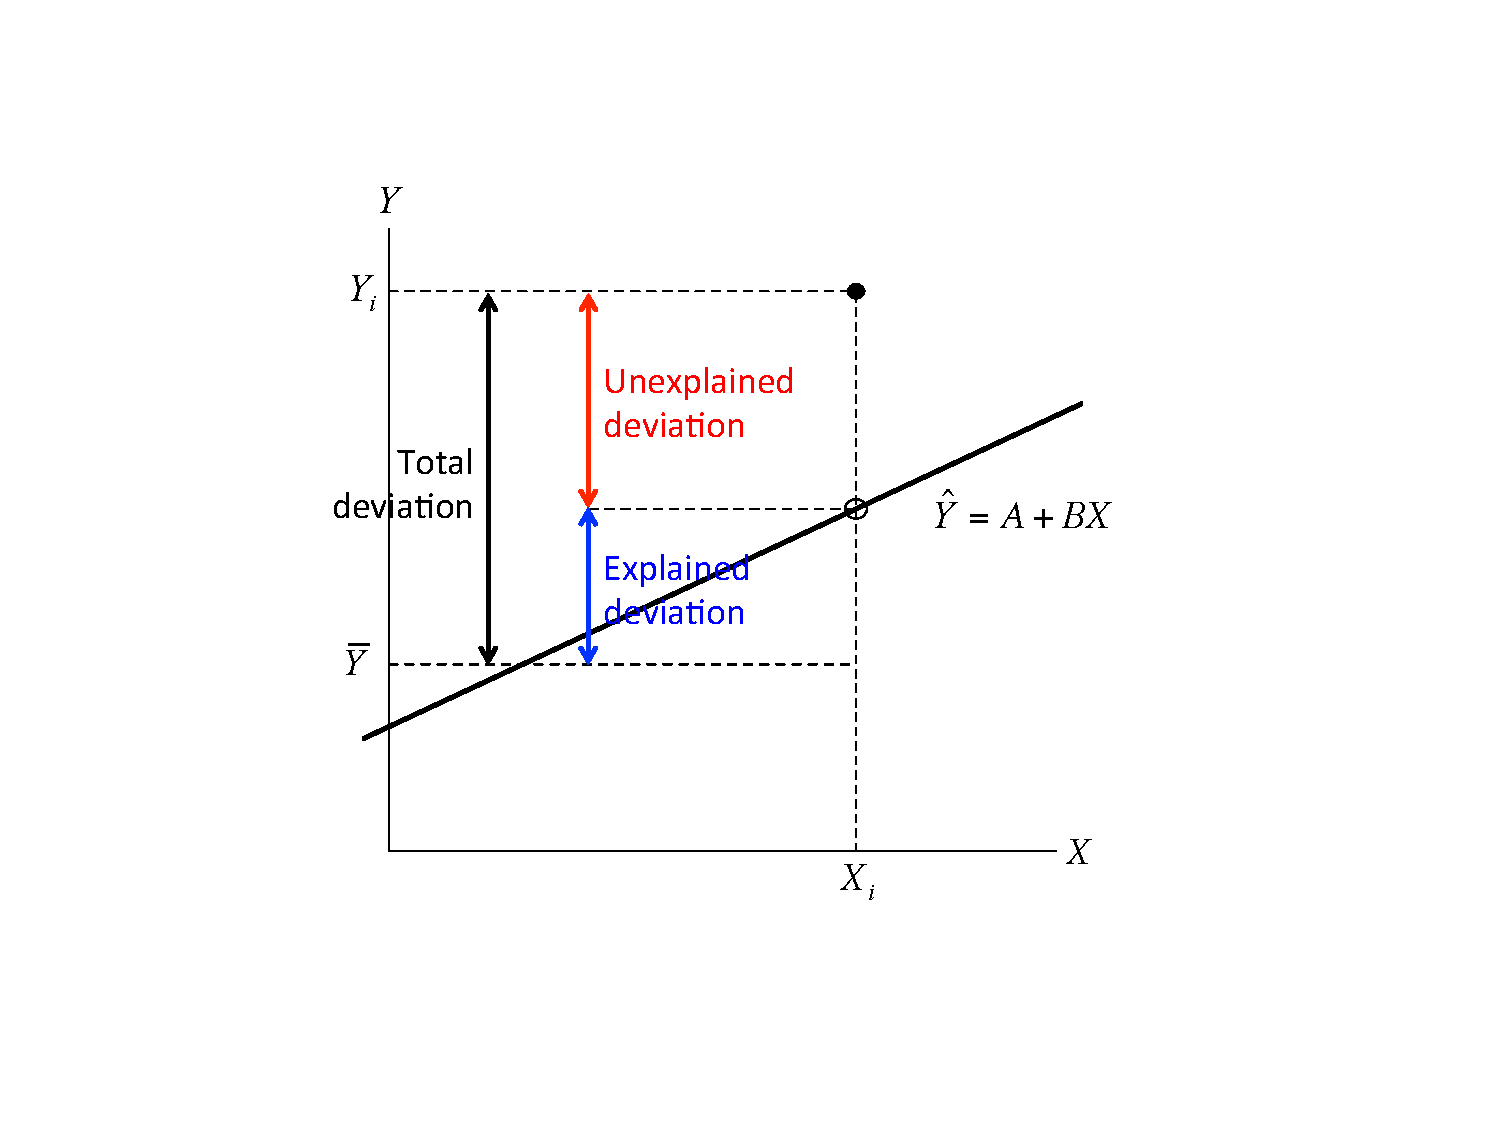
\includegraphics[width=5in]{../09_InterpretSimple/rsquared.pdf}%filename
  \caption{The Components of $R^{2}$ \label{fig:rsquared}}
\end{figure}

To calculate $R^{2}$ ``by hand" in \texttt{R}, we must first determine the total sum of squares, which is the sum of the squared differences of the observed values of $Y$ from the mean of $Y$, $\Sigma(Y_{i}-\bar Y)^{2}$. Using \texttt{R}, we can create an object called \texttt{TSS}. 
\begin{knitrout}
\definecolor{shadecolor}{rgb}{0.969, 0.969, 0.969}\color{fgcolor}\begin{kframe}
\begin{alltt}
\hlstd{TSS} \hlkwb{<-} \hlkwd{sum}\hlstd{((ds.omit}\hlopt{$}\hlstd{glbcc_risk}\hlopt{-}\hlkwd{mean}\hlstd{(ds.omit}\hlopt{$}\hlstd{glbcc_risk))}\hlopt{^}\hlnum{2}\hlstd{)}
\hlstd{TSS}
\end{alltt}
\begin{verbatim}
## [1] 23678.85
\end{verbatim}
\end{kframe}
\end{knitrout}
Remember that $R^{2}$ is the ratio of the explained sum of squares to the total sum of squares (\textit{ESS/TSS}). Therefore to calculate $R^{2}$ we need to create an object called \texttt{RSS}, the squared sum of our model residuals. 
\begin{knitrout}
\definecolor{shadecolor}{rgb}{0.969, 0.969, 0.969}\color{fgcolor}\begin{kframe}
\begin{alltt}
\hlstd{RSS} \hlkwb{<-} \hlkwd{sum}\hlstd{(ols1}\hlopt{$}\hlstd{residuals}\hlopt{^}\hlnum{2}\hlstd{)}
\hlstd{RSS}
\end{alltt}
\begin{verbatim}
## [1] 15431.48
\end{verbatim}
\end{kframe}
\end{knitrout}
Next, we create and object called \texttt{ESS}, which is equal to TSS-RSS.
\begin{knitrout}
\definecolor{shadecolor}{rgb}{0.969, 0.969, 0.969}\color{fgcolor}\begin{kframe}
\begin{alltt}
\hlstd{ESS} \hlkwb{<-} \hlstd{TSS}\hlopt{-}\hlstd{RSS}
\hlstd{ESS}
\end{alltt}
\begin{verbatim}
## [1] 8247.376
\end{verbatim}
\end{kframe}
\end{knitrout}
Finally, we calculate the $R^{2}$. 
\begin{knitrout}
\definecolor{shadecolor}{rgb}{0.969, 0.969, 0.969}\color{fgcolor}\begin{kframe}
\begin{alltt}
\hlstd{R2} \hlkwb{<-} \hlstd{ESS}\hlopt{/}\hlstd{TSS}
\hlstd{R2}
\end{alltt}
\begin{verbatim}
## [1] 0.3483013
\end{verbatim}
\end{kframe}
\end{knitrout}
Note--happily--that the $R^{2}$, calculated by ``by hand" in \texttt{R} matches the results provided by the \texttt{summary} command.

The values for $R^{2}$ can range from zero to 1. In the simple regression case, a value of 1 indicates that the modeled coefficient ($B$) "accounts for" all of the variation in $Y$. Put differently, all of the squared deviations in $Y_{i}$ around the mean ($\hat{Y}$) are in ESS, with none in the residual (RSS).\footnote{Note that with a \textbf{bivariate model}, $R^{2}$ is equal to the square of the correlation coefficient.} A value of zero would indicate that all of the  deviations in $Y_{i}$ around the mean are in RSS -- all residual or ``error". Our example shows that the variation in political ideology (our $X$) accounts for roughly 34.8 percent of the variation in our measure of perceived risk of global warming ($Y$). 

\noindent  \textbf{Visualizing Bivariate Regression}

The \texttt{ggplot2} package provides a mechanism for viewing the effect of ideology on the dependent variable of perceived risk of global warming. Adding \texttt{geom_smooth} will calculate and visualize a regression line that represents the relationship between yor IV and DV while minimizing the residual sum of squares.  Graphically (Figure \ref{fig:effectsplot}), we see as an individual becomes more conservative (ideology = 7), their perception of the risk of global warming decreases.

\begin{knitrout}
\definecolor{shadecolor}{rgb}{0.969, 0.969, 0.969}\color{fgcolor}\begin{kframe}
\begin{alltt}
\hlkwd{ggplot}\hlstd{(ds.omit,} \hlkwd{aes}\hlstd{(ideol, glbcc_risk))} \hlopt{+}
  \hlkwd{geom_smooth}\hlstd{(}\hlkwc{method} \hlstd{= lm)}
\hlkwd{dev.off}\hlstd{()}
\end{alltt}
\end{kframe}
\end{knitrout}

\begin{figure}[!htp]
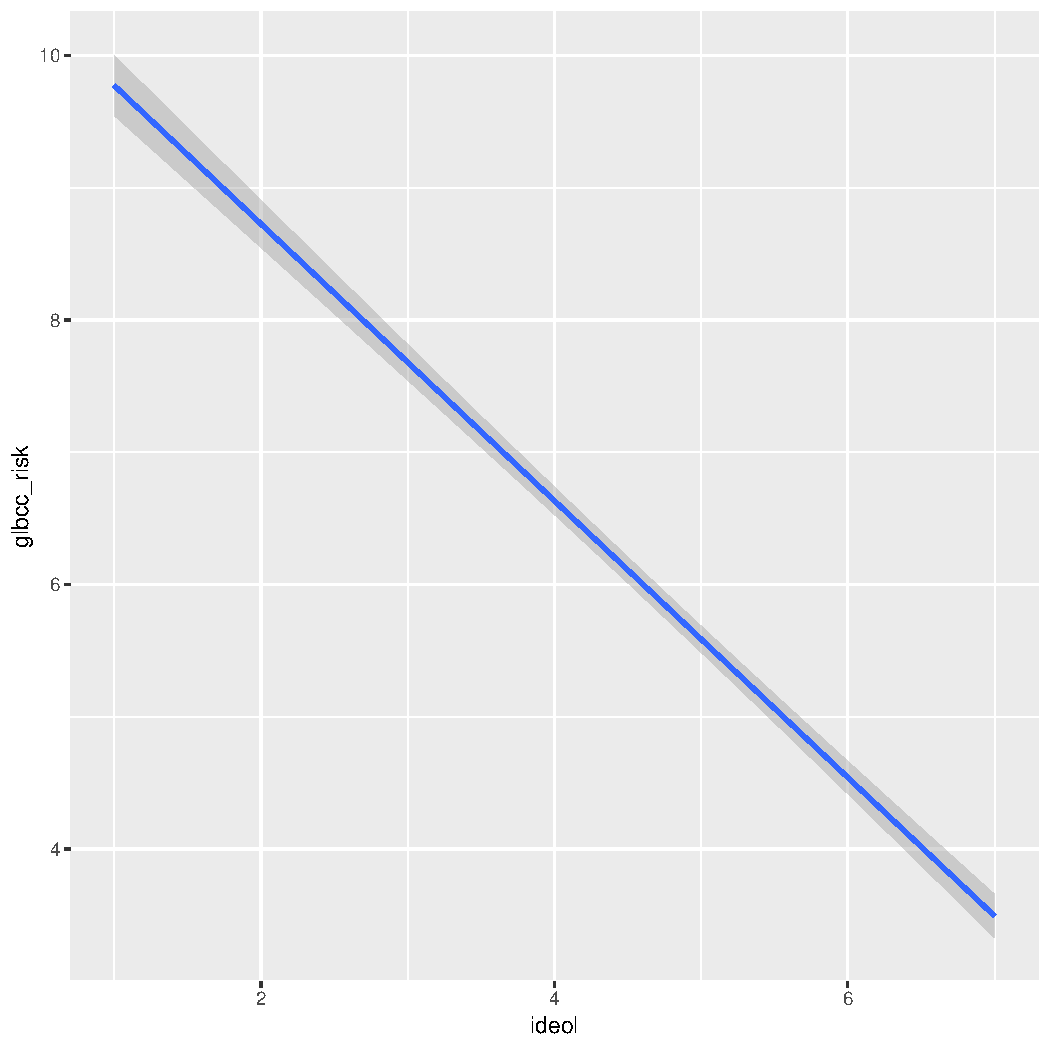
\includegraphics[width=3.5in, height=3.5in]{../09_InterpretSimple/effectsplot.pdf}%filename
\caption{Effects Plot of Ideology \label{fig:effectsplot}}
\end{figure} 

\noindent \textbf{Cleaning up the R Environment}

If you recall, at the beginning of the chapter, we created several temporary data sets.  We should take the time to clear up our workspace for the next chapter.
\begin{knitrout}
\definecolor{shadecolor}{rgb}{0.969, 0.969, 0.969}\color{fgcolor}\begin{kframe}
\begin{alltt}
\hlcom{#  we can clean up from the temporary data sets for this chapter.}
\hlkwd{rm}\hlstd{(ds.omit)} \hlcom{#remove the omit data set}
\end{alltt}
\end{kframe}
\end{knitrout}

\section{Summary} 

This chapter has focused on two key aspects of simple regression models -- hypothesis testing and  measures of the goodness of model fit. With respect to the former, we focused on the residual standard error, and its role in determining the probability that our model estimates, $B$ and $A$, are just random departures from a population in which $\beta$ and $\alpha$ are zero. We showed, using \texttt{R}, how to calculate the residual standard errors for $A$ and $B$ and, using them, to calculate the t-statistics and associated probabilities for hypothesis testing. For model fit, we focused on model covariation and correlation, and finished up with a discussion of the coefficient of determination -- $R^{2}$. So now you are in a position to use simple regression, and to wage unremitting geek-war on those whose models are endowed with lesser $R^{2}s$.
\end{document}
